\section{Durchführung}
\label{sec:Durchführung}

Es wird die Filterkurve des Selektiv-Verstärkers bei der Güte 
$G=\num{100}$ bestimmt. 
Anschließend bestimmt man mit der Apparatur in Abb. \ref{<++>} die 
Suszeptibilität von Oxiden einiger Seltener-Erd-Elemente. 


\subsection{Verfahren zur Unterdrückung der Störspannung}
Die Störspannung ist problematisch bei der Messung der Brückenspannung $U_\text{Br}$. 
Die Brückenspannung wird von der Störspannung komplett überdeckt, aber da die Signalspannung 
eine monofrequente Spannung ist, lässt sich dieses Problem mittels eines 
Selektivverstärkers beseitigen. Dessen Filterkurve hat die Gestalt einer Glockenkurve. 
Interessant ist dabei die Güte $G$ des Verstärkers. 
Frequenzen, die nah an der Frequenz $\nu_0$ liegen, werden nicht rausgefiltert, aber um 
Messungen zur Suszeptibilität an paramagnetischen Proben durchzuführen reicht der Filter. 

Es wird eine Schaltung wie in Abb. \ref{abb:schaltbild} benutzt, um die 
entsprechenden Spannungen herauszufiltern. 
Es wird also die Druchlassfrequenz des Selektivverstärkers auf die Signalfrequenz 
eingestellt. Anschließend wird die Brückenschaltung konfiguriert. Anschließend wird eine 
Probe in die Zylinderspule eingeführt. Die neue Brückenspannung wird genutzt um die 
Suszeptibilität zu berechnen. Das einzige was dann noch fehlt ist die Gesamtverstärkung 
der Apparatur, die abgelesen werden muss. 

\begin{figure}
    \centering
    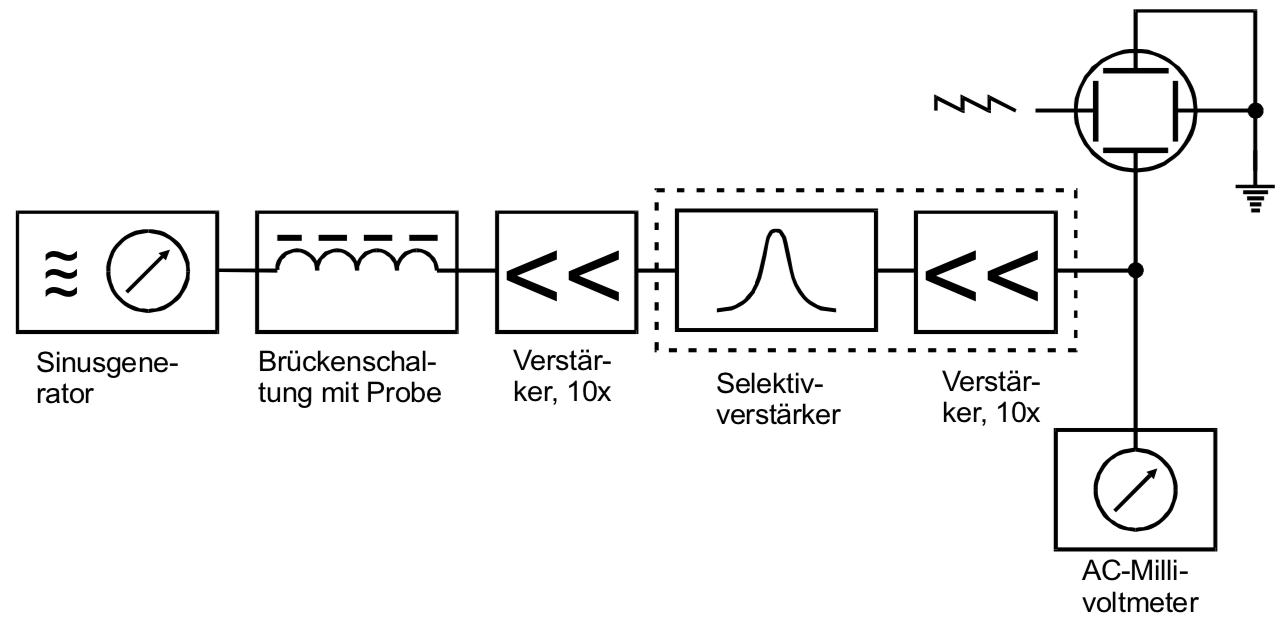
\includegraphics[width=15cm, height=7cm]{build/schaltbild.png}
    \caption{Schaltung zur Bestimmung der Suszeptibilität. \cite{V606}}
    \label{abb:schaltbild}
\end{figure}

\begin{figure}
    \centering
    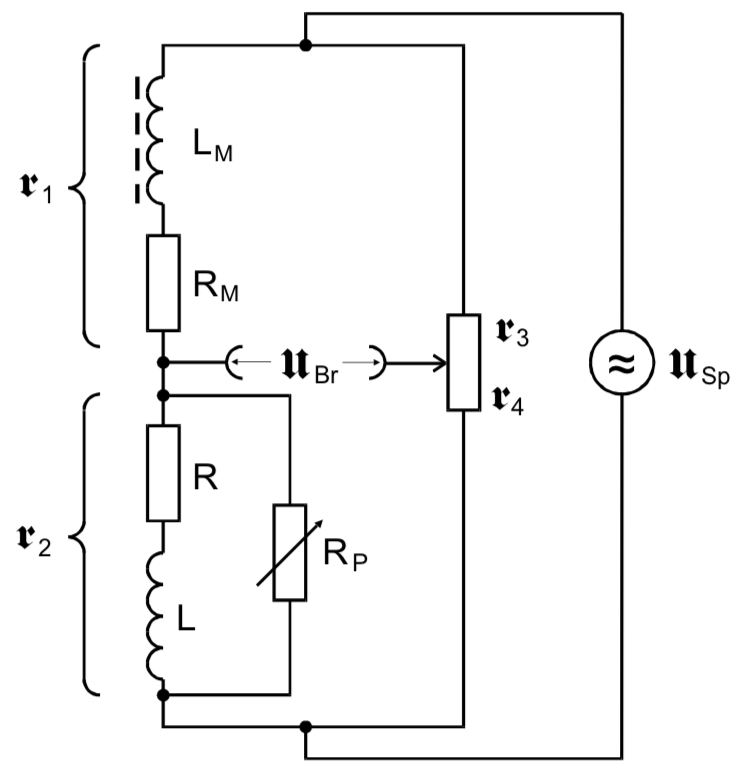
\includegraphics[width=10cm, height=12cm]{build/brueckenschaltung.png}
    \caption{Brückenschaltung zur Bestimmung der Suszeptibilität. \cite{V606}}
    \label{abb:brueckenschaltung}
\end{figure}